\chapter{Конструкторская часть}

\section{Требования к программному обеспечению}

Программа должна предоставить следующие функции:
\begin{itemize}
    \item создание сцены заданного размера;
    \item добавление, поворот, удаления объектов сцены;
    \item перемещение, поворот камеры сцены.
\end{itemize}

\section{Алгоритм, использующий z-буфер}

На рисунке \ref{img:zbuf} представлена схема алгоритма для удаления 
невидимых линий и поверхностей с помощью z-буфера. 

\clearpage
\begin{figure}[h]
    \centering
    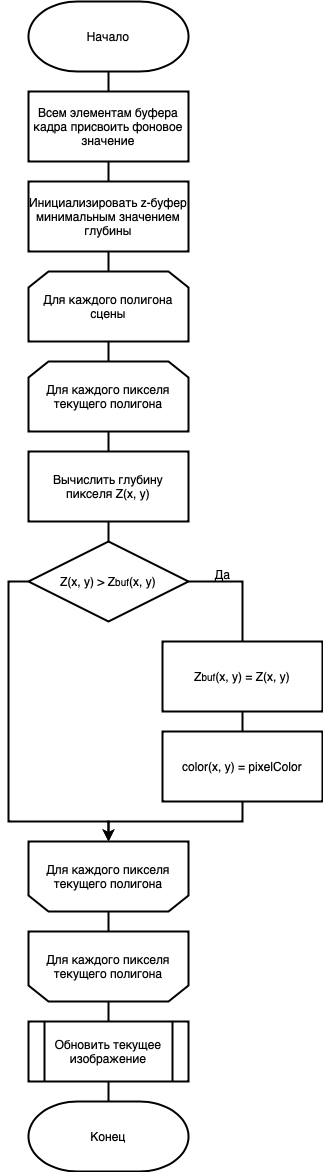
\includegraphics[width=0.4\linewidth]{img/zbuf.png}
    \caption{Схема алгоритма, использующего z-буфер}
    \label{img:zbuf}
\end{figure}
\noindent

\clearpage

\section{Алгоритм для построения теней, использующий z-буфер}

На рисунках~\ref{img:shadow1} -- \ref{img:shadow2} представлена схема алгоритма для построения теней с помощью z-буфера.

\begin{figure}[h]
    \centering
    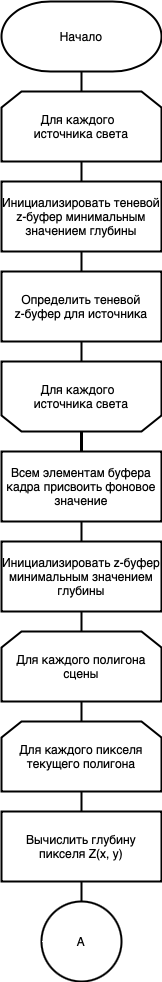
\includegraphics[width=0.23\linewidth]{img/shadow1.png}
    \caption{Схема алгоритма для построения теней, использующего z-буфер}
    \label{img:shadow1}
\end{figure}
\noindent

\begin{figure}[h]
    \centering
    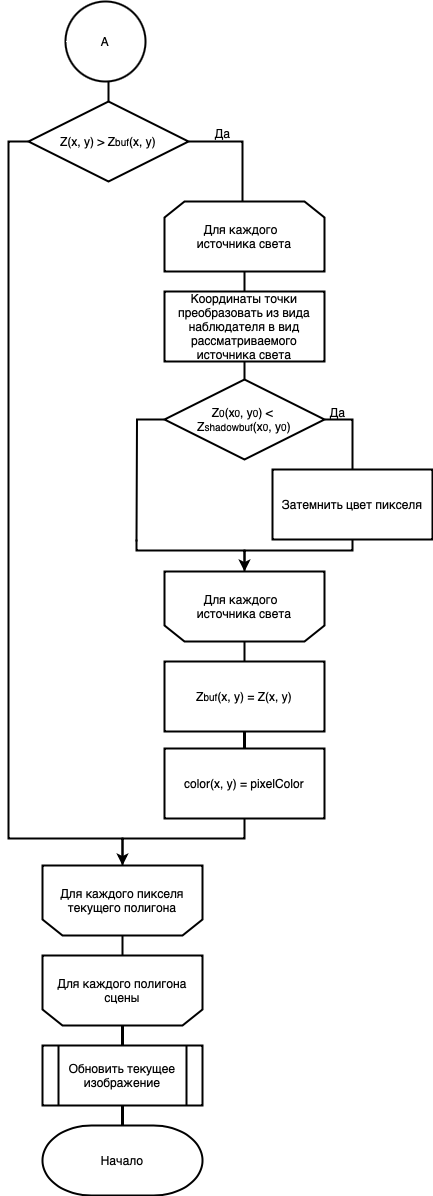
\includegraphics[width=0.5\linewidth]{img/shadow2.png}
    \caption{Схема алгоритма для построения теней, использующего z-буфер}
    \label{img:shadow2}
\end{figure}
\noindent

\clearpage
\section{Используемые типы и структуры данных для представления объектов}

Для решения поставленных задач курсового проекта необходимо опре- делить представление объектов разрабатываемой программы. 
В таблице \ref{tab:object} представлены объекты и выбранные для них типы и структуры данных.

\begin{table}[!ht]
    \centering
    \caption{\label{tab:object}Выбранный типы и структуры данных для представления объектов}
    \begin{tabular}{|p{6cm}|p{10cm}|}
    \hline
        Объект & Типы и структуры данных \\ \hline
        Точка в трехмерном пространстве & Вектор, состоящий из трех координат типа float64: x, y, z  \\ \hline
        Вершина & Точка в трехмерном пространстве \\ \hline
        Полигон & Структура, содержащая три вершины \\ \hline

        Камера &  Структура, содержащая направление и матрицу преобразования вершины
        в пространство камеры вершины в пространство камеры типа float64 \\ \hline

        Двигатель программы &  Структура, содеражащая: камеру,
        источник света, z-буфер, теневой буфер, 
        матрицу преобразования из пространства
        камеры в пространство исочника света типа float64\\ \hline
    \end{tabular}
\end{table}

\section*{Вывод}
В этом разделе были определены требования к программному обеспечению, выбраны типы и структуры данных. Также были разработаны 
алгоритм для удаления невидимых линий и поверхностей, использующий z-буфер и алгоритм, для построения теней с помощью z-буфера.
